\documentclass{article}
\usepackage[T1]{fontenc}
\usepackage[utf8]{inputenc}
\usepackage[margin=1in]{geometry}
\usepackage{fancyhdr} 
\usepackage{listings}
\usepackage{xcolor}

\definecolor{keywordcolor}{rgb}{0.4, 0.7, 1.0} % Light blue for keywords
\definecolor{ndkeywordcolor}{rgb}{0.8, 0.5, 0.0} % Orange for non-default keywords
\definecolor{stringcolor}{rgb}{0.8, 0.2, 0.2} % Red for strings
\definecolor{commentcolor}{rgb}{0.6, 0.6, 0.6} % Gray for comments
\definecolor{bracecolor}{rgb}{0.6, 0.6, 1.0} % Custom color for braces

\lstdefinelanguage{JavaScript}{
  keywords={break, case, catch, continue, debugger, default, delete, do, else, finally, for, function, if, in, instanceof, new, return, switch, this, throw, try, typeof, var, void, while, with},
  keywordstyle=\color{keywordcolor}\bfseries,
  ndkeywords={class, export, boolean, throw, implements, import, this},
  ndkeywordstyle=\color{ndkeywordcolor}\bfseries,
  identifierstyle=\color{black},
  sensitive=false,
  comment=[l]{//},
  morecomment=[s]{/*}{*/},
  commentstyle=\color{commentcolor}\itshape,
  stringstyle=\color{stringcolor}\ttfamily,
  morestring=[b]',
  morestring=[b]",
  literate={\{}{{\textcolor{bracecolor}{\{}}}1
           {\}}{{\textcolor{bracecolor}{\}}}}1
           {<}{{\textcolor{bracecolor}{<}}}1
           {>}{{\textcolor{bracecolor}{>}}}1,
}
\lstdefinelanguage{Python3}{
  keywords={False, async, class, finally, is, return, None, continue, for, lambda, try, True, def, from, nonlocal, while, and, del, global, not, with, as, elif, if, or, yield, assert, else, import, pass, break, except, in, raise},
  keywordstyle=\color{blue}\bfseries,
  ndkeywords={self},
  ndkeywordstyle=\color{darkgray}\bfseries,
  identifierstyle=\color{black},
  sensitive=true,
  comment=[l]{\#},
  morecomment=[s]{"""}{"""},
  commentstyle=\color{purple}\ttfamily,
  stringstyle=\color{red}\ttfamily,
  morestring=[b]',
  morestring=[b]",
  emph={print, len, range, int, str, float, list, dict, set, tuple},
  emphstyle={\color{teal}}
}
\usepackage[ruled,vlined]{algorithm2e}
\usepackage{amsthm}
\usepackage{amsfonts}
\usepackage{amssymb}
\usepackage{graphicx}
\usepackage[dvipsnames]{xcolor}
\usepackage{xy}
% \usepackage{url} % Commented out because hyperref provides similar functionality
\usepackage{parskip}
\usepackage{comment}
\usepackage{setspace}
\usepackage{enumerate}
\usepackage{multirow}
\usepackage{hyperref}
\usepackage{caption}
\usepackage{subcaption}
\usepackage{booktabs}
\usepackage{wrapfig}
\usepackage{times}

\captionsetup[figure]{font={small,it}}

\usepackage[backend=biber,style=numeric,sortcites,maxbibnames=99]{biblatex}
\addbibresource{references.bib}

\newcommand{\HRule}{\rule{\linewidth}{0.5mm}}
\newcommand{\Hrule}{\rule{\linewidth}{0.3mm}}
\newcommand{\classnum}{CS-GY 6313 B}

\makeatletter% since there's an at-sign (@) in the command name
\renewcommand{\@maketitle}{%
  \parindent=0pt% don't indent paragraphs in the title block
  \centering
  {\Large \bfseries\textsc{\@title}}
  \HRule\par%
  \textit{\@author \hfill \classnum}
  \par
}
\makeatother% resets the meaning of the at-sign (@)

\title{Assignment 4: Data Viz for Advocacy} 
\author{Ivan Aristy — iae225}
% \classnum

\begin{document}
  \maketitle % prints the title block
  \thispagestyle{empty}
  % \vspace{-15pt}

\section{Interactive Visualization}

\subsection{Question}
\label{subsec:subsec1}

\textbf{How are men's mental states in the US?}

The question is a bit general, but I want to communicate to a general audience
that is not aware of the high levels of mental health issues that men face in the US.

\subsection{Data}
\label{subsec:subsec2}

\subsubsection{Data Source}
\label{subsubsec:Data Source}

There are a few data sources to get information from.

The CDC holds lots of information, but particularly I looked into:

\begin{enumerate}
  \item Behavioral Risk Factor Surveillance System (BRFSS) Survey
  \item Household Pulse Survey
  \item National Health and Nutrition Examination Survey (NHANES)
  \item National Health Interview Survey (NHIS)
\end{enumerate}

However, much to my dismay, lot's of the Data I was looking for 
was not available. I was able to retrieve information for suicide rates,
but the data regarding mental health for men was quite limited or obscure.

I ended up using \url{https://www.cdc.gov/suicide/facts/data.html#cdc_data_surveillance_section_4-suicide-rates}
for suicide rate information, and \url{https://www.apa.org/monitor/2015/12/numbers}
for general information and stats regarding suicide rates.

\subsubsection{Serving Information} 
\label{subsubsec:Serving Backend Server}

For serving information, we use D3's csv function:

\begin{lstlisting}[language=JavaScript]
  import * as d3 from "d3";
  import { Dataset } from "@/types/types";
  import theme from "@/types/themes";
  
  export async function loadRatesData(): Promise<Dataset[]> {
    const data = await d3.csv("/rates.csv", d3.autoType); 
    console.log(data); 
  
    return [
      {
        label: "Total Population",
        data: data.map((d: any) => ({ x: d["Year"],
         y: d["Total Population"] })), 
        color: "#d4c2d4", 
      },
      {
        label: "Male",
        data: data.map((d: any) => ({ x: d["Year"], y: d["Male"] })),
        color: "#cbd4c2", 
      },
      {
        label: "Female",
        data: data.map((d: any) => ({ x: d["Year"], y: d["Female"] })), 
        color: "#c2c2d4", 
      },
    ];
  }  
\end{lstlisting}

and pass the data to the chart component through a wrapper.

\subsection{Visualization}
\label{subsec:Visualization}

\subsubsection{Frontend Setup}
\label{subsubsec:Frontend}

The frontend is a simple NextJS application that uses the 
\texttt{D3} library to create the chart, and react hooks to update 
and keep track of state.

My main secondary goal for this visualization was to make the 
design look sleek and simple. 

As opposed to my previous visualization, I wanted to make a website that
was more visually appealing and easier to understand, as well as having 
goodies like smooth transitions and a responsive design.

For smooth transitions I used the Lenis library, which allowed for smooth 
scrolling. This greatly improved the feel of the website, and allowed me 
to dynamically render the chart when the user scrolls to the chart section.

\begin{lstlisting}[language=JavaScript]
const [isVisible, setIsVisible] = useState(false);
    const ref = useRef<HTMLDivElement>(null);
  
    // Lenis hook to listen for scroll events
    useLenis(() => {
      if (ref.current && !isVisible) {
        const { top, bottom } = ref.current.getBoundingClientRect();
        const windowHeight = window.innerHeight;
  
        if (top + 300 < windowHeight && bottom > 0) {
          setIsVisible(true);
        }
      }
    });
\end{lstlisting}

To further my secondary goal, i carefuly created a color scheme that was
easy on the eyes, sleek, and modern. Also, I utilized DaisyUI to create 
components with a modern look and the color scheme described above:

\begin{lstlisting}[language=JavaScript]
  daisyui: {
    themes: [
      {
        mytheme: {
          primary: "#50514F",
          secondary: "#CBD4C2",
          accent: "#CF8E80",
          neutral: "#540D6E",
          "base-100": "#FFFCFF", // Background
          info: "#CBD4C2",
          success: "#CF8E80",
          warning: "#FFFCFF",
          error: "#540D6E",
        },
      },
    ],
  }
\end{lstlisting}

\subsubsection{Additional Components}
\label{subsubsec:Components}

The main page has a Hero component, a CTA, and data callouts.

The Hero displays the main question.

The CTA displays a button that takes the user to 
\url{https://www.mensmindsmatter.org/} to learn more about the topic
and how to get involved with donating.

\textbf{The final components are the data callouts}, which display some key insights
about men's health. I wish this could have been charts instead,
but finding specific information about mental health was a bit difficult.
Nevertheless, these prove helpful to the user to get informed on the topic.

\subsubsection{Visualization Logic}
\label{subsubsec:Visualization Logic}

I revisited D3 to create a custom chart, building upon my previous 
experience with the library. 

Working directly with D3 again proved to be more challenging 
but also rewarding, as it deepened my understanding of chart components 
and their implementation.

I gained a more explicit appreciation for the building blocks of a chart:

\begin{itemize}
  \item Margins: Carefully planned margins to ensure sufficient space for elements like axes, labels, and legends.
  \item Scales: Mapped dynamically to the data, ensuring that the chart is responsive to changes in data.
  \item Line: This time, I used 3 lines to represent the data, each with a different color.
  \item Tooltip: On hover, the user can see the exact data point they are looking at.
  \item Circles: Since we were using 3 lines and transitions, the circles also follow the lines created.
  \item Dynamics: I progresively drew the lines, and added a transition to make the chart more visually appealing. 
  I also believe that this draws attention to the chart, as the user is more likely to notice the chart if it is moving.
  Plus it highlights how rates increase over time.
  \item Axes: Created axes and basic labels for intuitive and fast understanding by the user.
\end{itemize}

\begin{figure}[ht] 
  \centering
  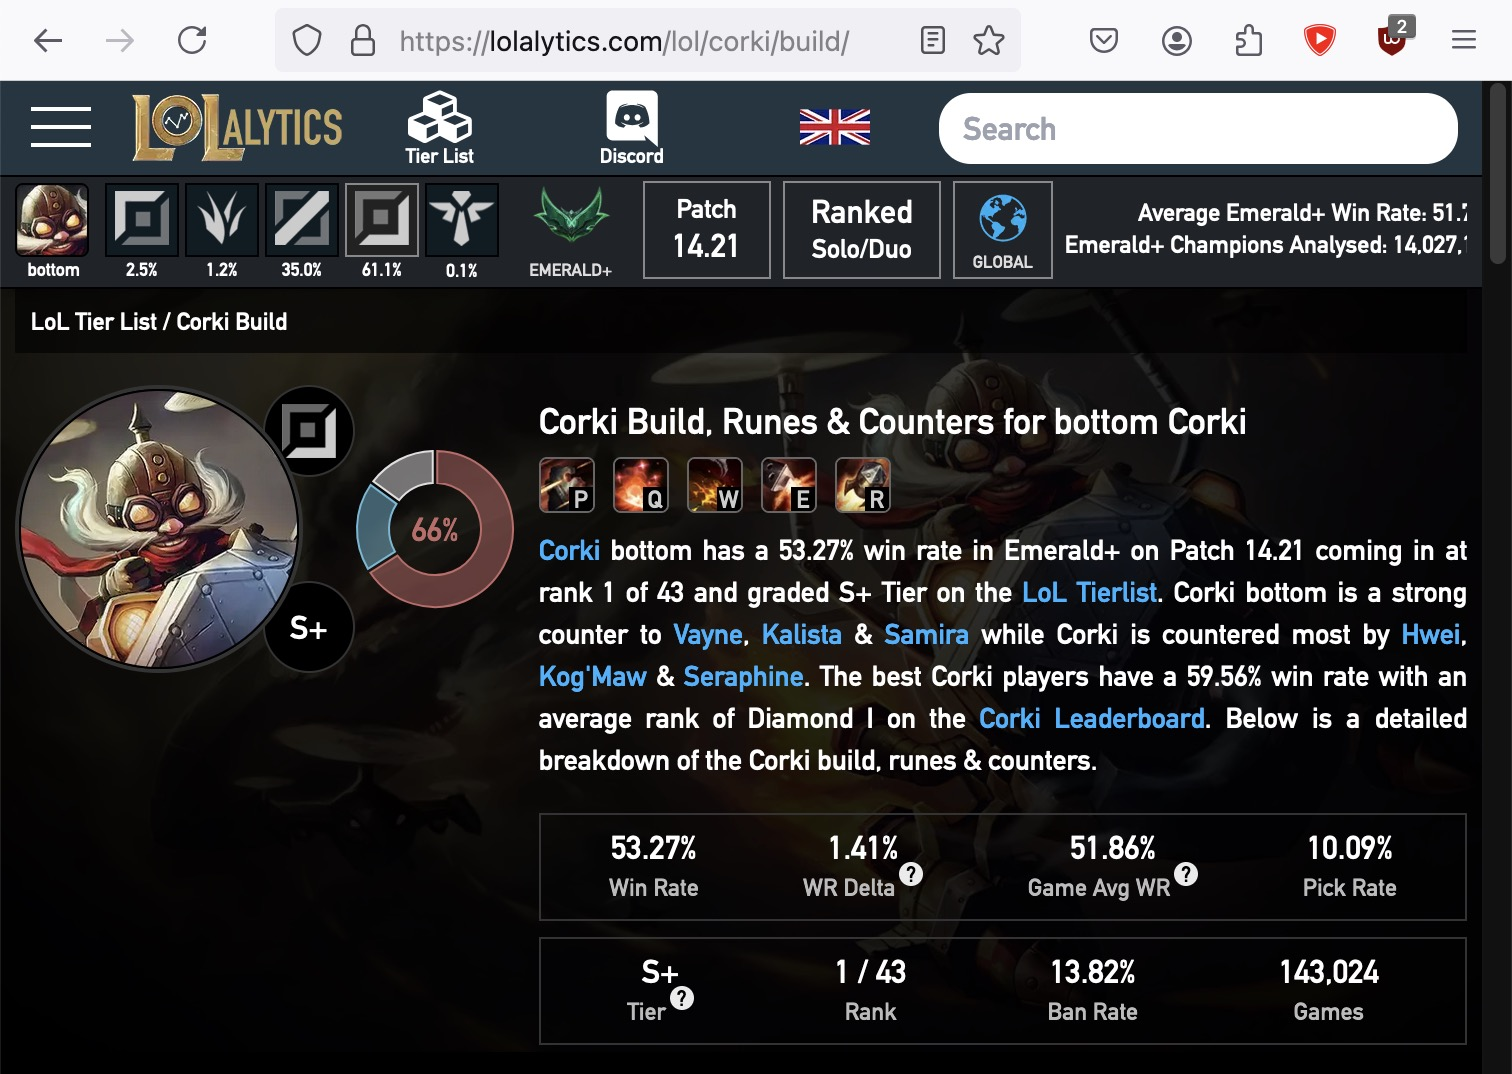
\includegraphics[width=0.75\textwidth]{figs/website.jpg}
  \caption{
      Corki's champion page.
  }
  \label{fig:fig1}
\end{figure}

\subsection{Improvements}
\label{subsec:Improvements}

\subsubsection{More Charts}
\label{subsubsec:Champion Image}

I would have liked to have more charts, but I was unable to aquire relevant data.

In the future, I would like to have a chart that shows the rates of mental
health issues posed by men. This would be a more direct visualization of the
trends, and how it's becoming a bigger and bigger issue. 

\subsection{Conclusion: Do we answer the question?}
\label{subsec:Conclusion}

I believe for both:


\begin{refcontext}[sorting=nyt]
\printbibliography
\end{refcontext}

\end{document}

